\chapter{Aplikovaná kybernetika [AKSZ]}

\section{Umělá inteligence [UI]}

\begin{table}[H]
\centering
\begin{tabular}{p{4cm} p{12cm}}
\textit{vyučující:}             & Prof. Ing. Josef Psutka, CSc. \\
								 & Ing. Aleš Pražák, Ph.D. \\
\textit{ročník/semestr studia:} & 2.ročník/ZS \\
\textit{datum zkoušky:}         & X. X. 2012 \\
\textit{hodnocení:}             & 1 \\
\textit{cíl předmětu (STAG):}   & \\
\multicolumn{2}{p{16cm}}{Cílem předmětu je seznámit studenty se základními problémovými oblastmi umělé inteligence (UI) a naučit je aplikovat vybrané metody řešení úloh, reprezentace znalostí v UI a hraní her.}
\end{tabular}
\end{table}

\subsection{Metody řešení úloh v UI}

\newpage
\subsection{Logické formalizmy pro reprezentaci znalostí. Predikátový počet 1. řádu. Rezoluční metoda.}

\newpage
\subsection{Produkční systém. Báze znalostí a báze dat. Dopředné a zpětné šíření.}

\newpage
\subsection{Síťové formalizmy pro reprezentaci znalostí. Sémantické sítě. Rámce. Scénáře.}

\newpage
\subsection{Metody hraní her v UI. Procedura minimax, alfa-beta prořezávání.}

\newpage
\section{Modelování a simulace 1 [MS1]}

\begin{table}[H]
\centering
\begin{tabular}{p{4cm} p{12cm}}
\textit{vyučující:}             & Ing. Václav Hajšman, Ph.D. \\
								 & Ing. Jindřich Liška, Ph.D. \\
								 & Ing. Miloš Fetter \\
\textit{ročník/semestr studia:} & 2.ročník/ZS \\
\textit{datum zkoušky:}         & X. X. 2012 \\
\textit{hodnocení:}             & 1 \\
\textit{cíl předmětu (STAG):}   & \\
\multicolumn{2}{p{16cm}}{Cílem předmětu je seznámit studenty se základními principy modelování dynamických systémů.}
\end{tabular}
\end{table}

\subsection{Systém, model, modelování, simulace, systémová analýza.}
\subsubsection*{Systém}
Objekty reálného světa jsou složité, těžko pozorovatelné. Pro studium objektů však máme určitý důvod, sledujeme určitý cíl a tedy nemusíme studovat objekty zcela obecně v plné složitosti – provádíme zjednodušení. Systémy jsou nástrojem studia objektů reálného světa, jsou zjednodušeným, abstraktním pohledem na objekty reálného světa. Systém je složitá entita tvořená vzájemně působícími prvky sloužící společnému účelu nebo podřízená společnému cíli (je-li podstata působení předávání informací, hovoříme o kybernetickém systému).
\begin{itemize}
\item \textit{Abstrakce}: zanedbání, vyloučení těch skutečností ze studia systému, které nejsou z hlediska sledovaného účelu (cíle) podstatné
\item \textit{Dekompozice}: rozklad systému na dílčí části – subsystémy a prvky
\item \textit{Hierarchie}: zachycení souvislostí mezi částmi systému vyjádřením sounáležitost částí systému ve smyslu nadřazenosti a podřízenosti, princip hierarchie v kombinaci s principem dekompozice vede k analýze systému od celku k částem, k postupnému, interaktivnímu zpřesňování a zjemňování popisu systému.
\item \textit{Modularita}: specifikace částí systému vykazujících jistou míru samostatnosti a minimální počet vzájemných vazeb
\end{itemize}

\subsubsection*{Model, modelování}
Jsou dány dva objekty X a Y a pozorovatel. Objektu X říkáme, že je modelem objektu Y, jestliže pozorovatel může použít objektu X k získání odpovědí na otázky, které se týkají objektu Y. Modelování není samostatným vědním oborem, jedná se o soubor principů, přístupů, metod k tvorbě modelů (definování systémů).

\subsubsection*{Simulační model, simulace}
Metoda získávání nových znalostí o systému na základě řízeného experimentování s jeho modelem. Simulační model – model určený (vhodný) pro simulaci (napodobení) chování reálného objektu. Provedeme-li nějaké řízené pozorování na reálném objektu, říkáme, že jsme provedli experiment. Provedeme-li takové řízené pozorování na modelu, označujeme ho simulací.
\begin{itemize}
\item \textit{Výhody}: cena, rychlost, bezpečnost, možnosti popisu velmi složitých systémů, u kterých by bylo použití jiných metod velmi složité nebo nemožné (například analytické řešení – aplikovatelné na jednoduché systémy nebo zjednodušené popisy složitých systémů)
\item \textit{Nevýhody}: náročnost tvorby simulačních modelů, problém ověření validity modelu, problém nepřesnosti a nestability numerických metod, výpočetní náročnost, jednorázovost
\end{itemize}
\vspace{3cm}
Vytvoření abstraktního modelu – formulace zjednodušeného popisu zkoumaného systému. Vytvoření simulačního modelu – zápis abstraktního modelu ve formě počítačového programu. Simulace – řízené experimentování se simulačním modelem.

\subsubsection*{Systémová analýza}
\begin{itemize}
\item \textit{izomorfní} vs. \textit{homomorfní} systémy: Izomorfní systémy jsou nerozlišitelné od sebe pro pozorovatele, který sleduje pouze jejich
vstupy a výstupy. Při homomorfismu existuje jednoznačné přiřazení mezi stavem systému A a B a nejednoznačné zpětné přiřazení – systém B získaný ze systému A zjednodušením, je homomorfním modelem systému A (shoda ve vybraných veličinách, nesymetrická relace). Vytváření homomorfních systémů je principem modelování, abstraktní model je homomorfní k modelovanému systému, simulační model je zpravidla izomorfní k abstraktnímu modelu.
\item \textit{spojité} vs. \textit{diskrétní} systémy: Dělení dle povahy interakce jejich prvků v čase.
\item \textit{bezsetrvačné} vs. \textit{dynamické} systémy: Dělení dle struktury. Dynamické systém obsahují setrvačnost (paměť) - např. integrátor, sekvenční logické obvody (sítě) vs. zesilovač, kombinační logické obvody
\item \textit{deterministické} vs. \textit{stochastické}: Dělení dle chování. U deterministických systémů jsou hodnoty proměnných v každém okamžiku přesně definovány, stochastické obsahují náhodu.
\end{itemize}

\subsection{Modelování systému diskrétních událostí, diskrétní simulace.}
Diskrétní simulace je simulace prováděná s diskrétními simulačními modely. V anglické literatuře se pro diskrétní simulaci používá výhradně termínu "discrete event
simulation", tedy simulace diskrétních událostí. Diskrétní simulační modely jsou modely diskrétní v čase i veličinách. Nejčastějším případem diskrétních modelů jsou aplikace teorie hromadné obsluhy.
\begin{itemize}
\item diskrétní v čase, časové okamžiky zpravidla neekvidistantní
\item diskrétní ve veličinách
\item stochastické chování
\item proměnný počet prvků systému
\item výskyt front reprezentovaných zpravidla spojovými seznamy
\item vysoký stupeň paralelismu a z toho vyplývající vysoké nároky na řízení programu
\end{itemize}

Událost je změna, jež je elementární a okamžitá (s nulovou dobou trvání). Události odpovídají diskrétním časovým okamžikům, v nichž se něco děje (dochází ke změně
stavu systému). Proces je posloupnost logicky na sebe navazujících událostí. Neprovádí se celý najednou, v jednom časovém okamžiku se provádí pouze část odpovídající právě jedné události (reakce na událost). Dílčí části procesu jsou od sebe odděleny tzv. plánovacími příkazy, které způsobí pozastavení procesu spojené s předáním řízení jinému procesu. Opětovná aktivace procesu vede k pokračování od místa posledního pozastavení.
\begin{itemize}
\item \textit{Aktivní}: Právě běžící proces, v daném okamžiku může být jen jeden
\item \textit{Ukončený}: Proces, který ukončil svoji operační část, nemůže být již nikdy aktivován
\item \textit{Pozastavený}: Proces naplánovaný k provedení v určitém čase, pokud nedojde ke zrušení zaplánování jiným procesem nebo nedojde k ukončení simulace, bude v tomto čase proveden
\item \textit{Pasivní}: Přímo (přímá aktivace) nebo nepřímo (prostřednictvím zaplánování) aktivovatelný proces jiným procesem
\end{itemize}
Plánování událostí je obecně vázáno na splnění určité podmínky (dosažení určité hodnoty simulárního času, dosažení určitého stavu modelovaného systému) - časové vs. podmínkové plánování. Nástroje: Simula, J-Sim, JavaSim, javaSimulation, ...

\subsection{Simulační experiment, studie, analýza rizika, náhoda v simulačních úlohách.}
\textit{Simulační pokus (experiment)}: Jeden experiment se simulačním modelem (fixované parametry simulačního modelu, fixovaná násada generátoru pseudonáhodných čísel).

\textit{Simulační studie}: Posloupnost simulačních pokusů majících stejný účel s cílem zjistit a analyzovat chování simulovaného systému při různých modifikacích nebo působení různých vlivů (proměnný určitý parametr simulačního modelu, fixovaná násada generátoru pseudonáhodných čísel).

\textit{Analýza rizika (posouzení relevantnosti, důvěryhodnosti získaných výsledků)}: 
\begin{itemize}
\item Posouzení vlivu změny parametru na získané výsledky.
\item Posouzení vlivu náhody na získané výsledky. Po nalezení optimální hodnoty parametru simulačního modelu provádíme ověřování vlivu náhody – měníme násadu generátoru pseudonáhodných čísel pro fixovanou hodnotu parametru simulačního modelu.
\end{itemize}
$ \mathrm{mira \, rizika} = \frac{\mathrm{pocet \, pokusu \, s \, I < I_{mez}}}{\mathrm{pocet \, vsech \, pokusu}} $, kde $ I_{mez} $ je mezní hodnota kritéria optimality.

\subsubsection*{Náhoda v simulačních úlohách}
Jednou ze základních charakteristických vlastností systémů diskrétních událostí je stochastický charakter chování. Simulační model musí tuto skutečnost respektovat $ \to $ nutnost specifikace základních parametrů stochastických procesů (příchody zákazníků, doby obsluh, poruchy, ...).
\begin{itemize}
\item Pro simulační modely koncepčních systémů (systémů definovaných nad fiktivními, neexistujícími objekty) – odhad získaný na základě zkušeností s chováním obdobných reálně existujících systémů
\item Pro simulační modely reálných systémů (systémů definovaných nad reálnými objekty) - odhad získaný na základě analýzy získaných experimentálních dat nebo jejich přímé využití
\end{itemize}
Implementace náhody v simulačním modelu, získání hodnot náhodných veličin:
\begin{itemize}
\item volba a parametrizace teoretické distribuční funkce, tj. funkce dané exaktním vzorcem (zpravidla využívána standardní rozložení pravděpodobnosti - normální, exponenciální, Poissonovo, rovnoměrné, ...)
\item specifikace empirické distribuční funkce (zpravidla schodovité nebo po částech lineární), jejíž hodnoty se získají analýzou experimentálních dat
\item přímé využití experimentálních dat
\end{itemize}
Diskrétní náhodné proměnné nabývají konečně nebo spočetně mnoho různých hodnot. U spojitých rozložení pravděpodobnosti hodnoty spojitě vyplňují určitý interval.

\subsection{Modelování v netechnických oborech (kompartmenty, buněčné automaty, ...).}
Speciální simulační techniky a nástroje - jednoduché účelově orientované prostředky pro řešení simulačních úloh v technické praxi a především v netechnických oborech. Popis reálného světa v logice a pojmech blízkých uživateli – odborníkovi z dané oblasti (biologie, lékařství, ...). Jejich užití nevyžaduje detailní znalosti z matematiky, programování, ... – problém řešen intuitivně v grafickém rozhraní. Pracovat se musí velmi opatrně, podmínky nikdy zcela neodpovídají reálným!

Dva přístupy k analýze a vytváření modelu:
\begin{itemize}
\item \textit{deduktivní}: potřeba přesné znalosti vyšetřovaných jevů a vstupních podmínek (teoretický přístup – problém!)
\item \textit{induktivní}: neznáme přesně fyzikální zákonitosti či nejsou odpovídající podmínky (medicína), jde o znalost dynamiky daného děje, ne o matematická pravidla
\end{itemize}

\subsubsection*{Techniky užívané v inženýrské biologii a lékařství}
\begin{enumerate}[label=(\alph*)]
\item \textit{Metoda řešení diferenční či diferenciální rovnice}
\begin{enumerate}[label=(\roman*)]
\item \textit{Forresterova (systémová) dynamika}: povaha problému - porodnost, úmrtnost (matematické rovnice se sestavují dle grafického zobrazení)
\item \textit{Ekvivalence elektrickým schématem}: vhodné pro modelování systémů, u kterých dochází k transportu látky v prostoru i času, např. nervové vlákno
\item \textit{Populační modely}: slouží k popisu populace, porovnávání a odhadu budoucího vývoje (nutnost matematického modelování); jednodruhové vs. vícedruhové
\item \textit{Epidemiologické modely}: modely časoprostorového šíření infekčních chorob - i pro modelování principiálně blízkých procesů; spojité (deterministické) vs. diskrétní v úrovni (stochastické)
\end{enumerate}
\item \textit{Kompartmentové modelování}: Popis zkoumaného systému prostřednictvím diskrétních oblastí (zón) mezi nimiž protéká kanály určitá látka. Rychlost změny určité látky v čase závisí na množství látky, jež do kompartmentu vstoupilo a vystoupilo (např. změny v endokrinním systému).
\begin{itemize}
\item Kompartment – diskrétní oblast (zóna) určitého systému, kterou je možné nějakým způsobem logicky či kineticky odlišit od okolí, homogenní
\item Kanály – propojení kompartmentů, kterými protéká určitá látka, jejíž dynamika nás zajímá, idealizujeme (nulový objem)
\item Vstup kompartmentu – reprezentován přivedením látky z jeho okolí nebo syntézou této látky uvnitř kompartment
\item Výstup kompartmentu – pohyb látky mimo prostor kompartmentu nebo její transformací do jiné formy
\end{itemize}
\begin{enumerate}[label=(\roman*)]
\item \textit{Modelování systému příjmu potravy}: Chceme sledovat dynamiku koncentrace nějaké látky, která je součástí potravy.
\item \textit{Modelování funkce ledvin}: Zbavování organismu nadbytečné vody.
\item \textit{Distribuce dýchacích plynů v organismu (1967)}: Kompartmenty propojeny cirkulující krví. 
\end{enumerate}
\item \textit{Celulární (buněčné) automaty}: Dynamické systémy s diskrétním prostorem a časem, které jsou charakterizovány čtyřmi základními vlastnostmi:
\begin{itemize}
\item Geometrií buněčné mřížky - zpravidla pravidelné N rozměrné soustavy buněk
\item Specifikací okolí buňky (von Neumann (4), Moor (8), rozšířený Moor (24), ...)
\item Množinou stavů buňky – často dvoustavové buňky (aktivní x neaktivní, živá x mrtvá)
\item Algoritmem vypočtu příštího stavu buňky na základě současného stavu této buňky a jejího okolí (pravidla)
\end{itemize}
Příklady: hra Life, šíření epidemie
\end{enumerate}

\subsection{Konstrukce modelů na základě měření, zpracování signálu v časové, frekvenční a časo-frekvenční oblasti, modely periodických procesů.}
\vspace{2.5cm}
\begin{itemize}
\item sledované veličiny: dynamické (krátkodobé) chování systému (dráha, rychlost, zrychlení)
\item provozní parametry: statické (dlouhodobé) chování systému (teplota, tlak, otáčky, ...)
\item analýza dat: určení stavu a vlastností systému v časové, frekvenční, časo-frekvenční oblasti
\item vyhodnocení dat: funkce hodnotící analyzovaná data; překročení určitého prahu ukazuje na změnu stavu sledovaného systému (alarm)
\end{itemize}
Dělení signálu: 
\begin{itemize}
\item deterministický (periodický vs. neperiodický) vs. stochastický (stacionární vs. nestacionární)
\item spojitý v čase vs. diskrétní v čase
\item spojitý v hodnotách vs. diskrétní v hodnotách
\end{itemize}
Deterministické signály lze popsat pomocí přesného analytického vyjádření. Pro periodické signály platí $ x(t) = x(t+T) $. Harmonické signály s konstantní frekvencí a amplitudou lze popsat vztahem $ x(t) = A sin \left( \frac{2 \pi}{T} t + \varphi \right) = A sin (2\pi f t + \varphi) $

\subsubsection*{Zpracování signálů v časové oblasti}
Základní charakteristiky:
\begin{itemize}
\item \textit{Energie signálu}: $ E = \displaystyle{\int_{-\infty}^\infty} |x(t)|^2 dt $. Signály s konečnou energií nazýváme energetické.
\item \textit{Výkon signálu}: $ P = \underset{T \to \infty}{\mathrm{lim}} \frac{1}{2T} \displaystyle{\int_{-\infty}^\infty} |x(t)|^2 dt $. Signály s konečným výkonem nazýváme výkonové (musí být periodické), ty lze dále charakterizovat stejnosměrnou složkou (bez abskv) a efektivní hodnotou ($ \sqrt{P} $).
\item \textit{Korelační funkce}
\begin{itemize}
\item autokorelační funkce: $ R(\tau) = \displaystyle{\int_{-\infty}^\infty} x(t) x(t+\tau) dt $. Autokorelační funkce periodického signálu je také periodická.
\item vzájemná korelační funkce: $ R_{xy}(\tau) = \displaystyle{\int_{-\infty}^\infty} x(t) y(t+\tau) dt $.  Ze vzájemné korelační funkce lze určit závislost dvou funkcí, např. posun v čase.
\end{itemize}
\end{itemize}

\subsubsection*{Zpracování signálů ve frekvenční oblasti}
Z časového průběhu často nelze získat dostatečné množství informace - změny vlastností systému jsou skryty v šumu pozadí (strukturální vibrace, akustické
rezonance, ...) $ \to $ parametrické metody pro odhad spektra – Burg, Yule-Walker (průměrování spekter - v diagnostice nejpoužívanější metoda ke snížení šumu ve spektru).
Pokud 1) počet nespojitostí signálu $ x(t) $ je konečný a 2) $ \displaystyle{\int_{0}^\tau}|x(t)| dt < \infty $, lze signál $ x(t) $ rozvinout v trigonometrickou řadu se základní frekvencí $ \omega = \frac{2\pi}{T} $ (lze ji zapsat také v komplexním tvaru).
\begin{equation}
x(t) = \frac{a_0}{2} + \displaystyle{\sum_{k=1}^\infty \left[ a_k cos(k\omega t) + b_k sin(k\omega t) \right]} = \frac{a_0}{2} + \displaystyle{\sum_{k=1}^\infty \left[ A_k cos(k\omega t + \varphi_k) \right]}
\end{equation}
Člen před sumou odpovídá stejnosměrné složce dané funkce (signálu). Harmonický člen pro $ k = 1 $ se nazývá první nebo základní harmonická a členům pro $ k > 1 $ říkáme vyšší harmonické. Hodnota $ A_k $ je amplitudou k-té harmonické a $ \varphi_k $ odpovídá počátečnímu fázovému posuvu dané harmonické.

\textbf{Fourierova transformace} je limitním případem Fourierovy řady pro neperiodické signály.
\begin{equation}
\boxed{X(\omega) = F[x(t)] = \displaystyle{\int_{-\infty}^\infty} x(t) e^{-j\omega t} dt}
\end{equation}
\begin{itemize}
\item linearita: $ F[ax(t) + by(t)] = aX(\omega) + bY(\omega) $
\item posun signálu v čase má vliv pouze na fázové spektrum: $ F[x(t-t_0)] = X(\omega)e^{-j\omega t_0} $
\item posun ve frekvenci: $ F[x(t)e^{j \omega_0 t}] = X(\omega-\omega_0) $
\item součin signálů odpovídá konvoluci jejich Fourierových obrazů: $ F[x(t) \cdot y(t)] = X(\omega) * Y(\omega) $
\item konvoluce signálů odpovídá součinu jejich Fourierových obrazů: $ F[x(t) * y(t)] = X(\omega) \cdot Y(\omega) $
\end{itemize}
Veškeré signály, které v praxi naměříme, mají konečnou délku (dáno trváním měření). Vzorkováním spojitého signálu získáme diskrétní signál definovaný v časových okamžicích $ x(kT_s) $. Diskrétní Fourierova transformace (\textbf{DFT}):
\begin{equation}
x \left[ \frac{n}{NT_s} \right] = T_s \displaystyle{\sum_{i=0}^{N-1}}x [kT_s]e^{-j\frac{2\pi k n}{N}}, \qquad k=0,1,...,N-1 
\end{equation}

\textbf{Analýza signálů ve frekvenční oblasti}: reálná diagnostická data z většiny procesů jsou ve své podstatě nejčastěji nestacionární, nelineární a příliš krátká (neopakovatelná). Fourierova transformace je obecná metoda pro analýzu celkového rozložení amplitudy v závislosti na frekvence, ale, systém musí být lineární, data musí být stacionární a nelze rozlišit puls a šum.

\subsubsection*{Zpracování signálů v časo-frekvenční oblasti}
Frekvenční analýza nestacionárních signálů, tj. signálů, jejichž parametry se mohou měnit v čase. Nutnou podmínkou pro korektní vyhodnocení výsledků DFT je právě neměnnost parametrů signálů a jeho periodicita. Jestliže signál není periodický, dochází k tzv. úniku ve spektru (prosakování ve spektru).

\textbf{Krátkodobá Fourierova transformace (STFT)} je vypočtena z krátkých úseků analyzovaného signálu:
\begin{equation}
X(t,\omega) = \displaystyle{\sum_{-\infty}^\infty} x(\tau)h(\tau-t)e^{-j\omega t}d\tau
\end{equation}
kde $ x(t) $ je analyzovaný signál a $ h(t) $ je okénková funkce (pravoúhlé, Hamming,...). Předpokladem je, že ten krátký úsek signálu, vzniklý převážením původního signálu okénkovou funkcí, je stacionární, tj., že se jeho parametry nemění. Amplitudové spektrum krátkodobé Fourierovy transformace lze zobrazit třeba spektrogramem. Umožňuje sledovat změnu amplitudy (energie) signálu v závislosti na frekvenci a čase, ale analýza je ovlivněna Heisenberg-Gaborovým principem neurčitosti.

\textbf{Wavelet transformace} využívá k dekompozici množinu ortonormálních funkcí (bází) a poskytuje analýzu s vícenásobným rozlišením (multiresolution) - použití okna proměnné délky s jednou vlnkou (waveletem) $ \to $ podrobnější časové rozlišení ve vyšších frekvencích (na úkor frekvenčního rozlišení). 

Dosud jsme se bavili o metodách lineární časo-frekvenční dekompozice. Mezi metody využívající okamžitou frekvenci patří Hilbertova-Huangova transformace a Kalmanův filtr.

\subsubsection*{Modely periodických procesů}
Rubbing je ve většině případů až důsledkem některé závady stroje. Mezi nejčastější příčiny rubbingu patří síly, které způsobují ohyb hřídele. Změna geometrie hřídele může vést ke kontaktu mezi rotorem a statorem. Zvýšením teploty v místě kontaktu dochází k dilataci kovového materiálu což způsobuje další průhyby hřídele. Druhou častou příčinou rubbingu jsou nadměrné vibrace, kdy jejich amplituda přesáhne povolenou mez mezi rotorem a statorem. K tomuto jevu může docházet například během přechodu stroje přes kritické otáčky, a jedná se o děj přechodný.

Projevy rubbingu:
\begin{itemize}
\item změna tuhosti spojení systému rotor-ložisko-stator $ \to $ změna přirozené frekvence, změna amplitudy a fáze
\item nárazy $ \to $ vznik sub-a super-synchronních komponent, vznik vysokofrekvenčních komponent, šum
\item tření $ \to $ vznik vysokofrekvenčních komponent, šum, povrchové opotřebení
\end{itemize}
Typy rubbingu: částečný vs. úplný. Typy úplného rubbingu:
\begin{itemize}
\item synchronní (s dopřednou precesí): Je buzen silou nevývažku rotoru. Precese rotoru je shodná se smyslem jeho otáčení okolo osy rotace.
\item samobuzený (se zpětnou precesí): Precese rotoru není shodná se smyslem otáčení rotoru okolo osy rotace. Může vzniknout v oblasti rezonanční 
\end{itemize}

\subsection{Modely vibrací a kmitání, experimentální modální analýza.}
\begin{enumerate}[label=(\alph*)]
\item \textbf{Statistické metody}
\begin{enumerate}[label=(\roman*)]
\item \textit{Činitel výkmitu - crest-faktor}: Metoda je založena na faktu, že periodicky se opakující vibrační ráz lze s postačujícím rozlišením vyhodnotit z výkmitu měřeného vibračního signálu. Tento výkmit je však prakticky neměřitelný jako efektivní hodnota v daném kmitočtovém rozsahu. Zhoršující se technický stav se projevuje nárůstem jak četnosti rázů tak jejich výkmitů. Efektivní hodnota vibračního signálu se zvětšuje se zvyšující se četností rázů, zatímco se hodnota výkmitů stabilizuje. Podíl mezi maximální a efektivní hodnotou vibrací (zrychlení). Vyhodnocuje se z časového signálu (frekvenční pásmo 10Hz – 10kHz): $ c_f = \frac{\hat{a}}{a_{eff}} $. Metoda je rychlá a laciná, ale není příliš přesná co se týče stanovení stupně poškození. Je navíc nevýhodná při parazitních zdrojích kmitů.

\item \textit{K-hodnota}: Zohledňuje efektivní a maximální (špičkové) hodnoty při stavu bez poškození a v aktuálním stavu: $ K(t) = \frac{a_{eff}(0) \cdot \hat{a}(0)}{a_{eff}(t) \cdot \hat{a}(t)} $. K tomu, aby mohlo být rozhodnuto o aktuálním stavu, jsou stanoveny hladiny parametru $ K(t) $, které vycházejí z dlouholetých zkušeností a poznatků. Metoda parametru K(t) je rychlá a nenáročná a oproti srovnatelným metodám spočívá její výhoda v diagnostikovatelnosti většího množství zdrojů poškození. Nebylo zjištěno omezení její platnosti.
\item \textit{Kurtosis}: Nespoléhá se na měření absolutní velikosti vibrací. Způsob výpočtu veličiny je je založen na rozdělení amplitud signálu: $ K = \frac{\int (x-x^{-4})p(x)dx}{\sigma^4} $. Nepoškozené ložisko emituje stochastické kmitání, které má gaussovo normální rozdělení
pravděpodobnosti a hodnota K pro toto rozdělení je K=3. Tuto hodnotu můžeme naměřit v širokém pásmu od 2,5 kHz do 80 kHz s odchylkami +- 8\% (nezávisle na zatížení a otáčkách). S postupujícím poškozením roste koeficient K v nižším frekvenčním pásmu. Velké poškození vede k nárůstu hodnoty K ve vyšších frekvencích, zatímco v nízkých frekvencích se koeficient K vrací zpět na svou původní hodnotu.Míra poškození určovaná Kurtosis faktorem se proto odhaduje v pěti frekvenčních pásmech.
\end{enumerate}
\item \textbf{Rezonanční metody} (rezonance snímače)
\begin{enumerate}[label=(\roman*)]
\item \textit{Metoda rázových pulsů (SPM/BCU)}: Princip spočívá v měření a posouzení rázových pulzů. V měřícím zařízení je signál filtrován pásmovou propustí se střední frekvencí pásma v okolí rezonanční frekvence snímače. (nejčastěji cca 35 kHz). K určení vlastního stavu je monitorována maximální hodnota špičky impulsu (shock value) v signálu, jejíž nárůst poukazuje na počínající poškození v drahách ložiska. V prahové hodnotě (carpet value) je shrnut vibrační šum ložiska. Nárůst této hodnoty zpravidla poukazuje na problémy s mazáním. Aby mohl být stav ložiska posuzován objektivněji a aby mohla být posuzována různá ložiska navzájem, je nutné provádět měření ložiska v dobrém stavu (nově osazené ložisko) a hodnoty metody normovat. Diference špičkové a prahové hodnoty se blíží svými vlastnostmi činiteli výkmitu (crest- factor).
\item \textit{Metoda špičkové energie (Spike Energy)}: Zpracováván je signál z akcelerometru v oblasti od 100 Hz až do 65 kHz. Dále je definována očekávaná frekvence poškození ložiska $ f_D $, požadovaný počet harmonických $ n_{SE} $, které budou k dispozici ve výsledném spektru. Pokud není nastavena očekávaná frekvence poškození $ f_D $, pak je pro další výpočet použita maximální frekvence $ f_{max} $ obsažená v měřeném signálu. Pro každý vzorek signálu z A/D převodníku se počítá odstup aktuálního vzorku od předchozího maximálního záporného impulsu. Pokud je hodnota aktuálního vzorku menší než hodnota maximálního záporného impulsu, pak bude maximální záporný impuls nastaven na tuto hodnotu. Odstup aktuálního vzorku od maximálního záporného impulsu je označován jako peak-to-peak a je v každém kroku násoben konstantou tlumení. \end{enumerate}
\item \textbf{Frekvenční metody}
\begin{enumerate}[label=(\roman*)]
\item \textit{Obálková analýza}: Metoda, kterou mohou být detekovány a monitorovány opakující se rázy již v raném stadiu jejich vzniku a vývoje. Velmi krátké a rychle doznívající pulsy nejsou rozpoznatelné přímou frekvenční analýzou
měřeného signálu. K tomu slouží vytvoření obálkové křivky časového signálu. Měřený signál je vlastně superpozicí vibračního signálu ložiska se stacionárním základním kmitáním a rovněž s cizími vibracemi, které se šíří materiálem z okolních částí stroje. Filtrace horní propustí, nebo pásmovou propustí proto, aby se odstranily vlivy například otáček rotoru a dalších složek, které se projevují v nízkých frekvencích. Signál na výstupu obsahuje jen složky s vysokými kmitočty, ke kterým zaručeně patří i kmitání, impulsy v důsledku rázů. Následně je filtrovaný signál usměrněn a filtrován dolní propustí. Tento postup odstraňuje nosný signál (vlastní kmitavé pohyby stroje) a výsledkem je obálka původního časového signálu. Signál obálky se dále analyzuje např. pomocí FFT ve frekvenčním spektru. 
\vspace{3cm}
\item \textit{Kepstrální analýza}: Slouží k rozpoznání periodicit ve frekvenčním spektru: $ c(\tau) = F[log[]F(x(t))[]] $ 
\end{enumerate}
\item \textbf{podíl KRMS/LRMS}: Podíl mezi krátkodobou a dlouhodobou efektivní hodnotou - pro ohodnocení navýšení intenzity signálu (odhalení nestacionarit z časového signálu). Při vzniku nestacionarity dojde k navýšení intenzity signálu a tím i k nárůstu efektivní hodnoty. Efektivní hodnota může ale vlivem změn stavu zařízení značně kolísat. Pro odstranění těchto relativně pomalých změn je krátkodobá efektivní hodnota K-RMS (Kurzzeit-RMS) dělena dlouhodobou efektivní hodnotou L-RMS (Langzeit-RMS). Délka okna LRMS je řádově větší než u KRMS (jedná se řádově o sekundy, kdežto okno KRMS je v řádu milisekund).
\end{enumerate}

Využití: monitoring volných částí v primárním okruhu JE, detekce pádu keramického obkladu ve spalovací komoře plynové turbíny, včasné určení poruchy ložiska.

Shrnutí:
\begin{itemize}
\item akcelerometry: senzory pro snímání vibrací
\item analýza vibračních signálů v časové a frekvenční oblasti odděleně je dobře použitelná v mnoha aplikacích, ale je vždy nutné zhodnotit jejich použití vzhledem k charakteru úlohy
\item časo-frekvenční analýza je důležitým nástrojem pro řešení problémů s analýzou nestacionárních a nelineárních signálů
\item v časo-frekvenční oblasti je možné selektivně analyzovat krátkodobé změny na určitých frekvencích a v určitém čase odděleně od rezonancí
\item pro potlačení nežádoucích frekvencí v zobrazení je používáno tzv. normování (adaptivní pro krátkodobé změny a na určitý stav systému pro dlouhodobé změny)
\end{itemize}

\subsubsection*{Experimentální modální analýza}
Cílem modální analýzy je určení vlastních frekvencí dílu nebo soustavy dílů (součástí mechanické konstrukce). Tyto vlastní frekvence slouží k informaci o měřeném objektu, které se potom využívají k hodnocení provozních stavů, kdy by případná rezonance některé z provozních frekvencí s vlastní frekvencí vedla k totálnímu zničení objektu. Možnost určení vlastních frekvencí jsou podle způsobu zjišťování: 1) \textit{výpočet} - teoretická (analytická modální analýza); 2) \textit{experiment} - experimentální modální analýza (modální zkouška).

Vytvoření matematického modelu popisujícího dynamické chování testované struktury experimentální cestou. Získáme: 1) vlastní frekvence, 2) modální tlumení, 3) vlastní tvar $ \to $ modální model (fyzikální/modální/odezvový).

\textit{Proč se provádějí modální zkoušky?} Většina průmyslových odvětví běžně navrhuje své struktury na počítačích a často mají jejich analytický model. Dynamické vlastnosti vypočítané pomocí tohoto modelu je potřeba ověřit pomocí modální zkoušky na prototypu $ \to $ doladění konečnoprvkového (MKP) modelu, snížení vibrací, simulace scénáře "co se stane, když..." (letecký, automobilový průmysl).

Shrnutí:
\begin{enumerate}
\item Vytvoření modelu pro modální zkoušku. Často už před zkouškou existuje počítačový geometrický model. Potom je úkolem definovat, které body na struktuře se mají měřit a ve kterých směrech. Tento krok je velmi důležitý, protože cílem je omezit množství měření a neprovádět zbytečnou, časově náročnou, přípravnou práci. Na druhé straně je však třeba vybrat správné body, aby byl vytvořen použitelný modální model. Často se použije část MKP modelu a výhodou je, že MKP analýza nám dává množství hodnotných informací pro tvorbu co nejlepšího modelu pro modální zkoušku.
\item Měření je často časově nejnáročnější krok. Čas zabírá instalace snímačů a jejich nastavení, což může často zabrat 80\% času celé zkoušky. Jak už bylo diskutováno, pro
prokládání křivek se používají frekvenční odezvové funkce, ale často jsou pro ověření důležité i jiné funkce. Můžeme zmínit koherenci, autospektrum aj.
\item Mnoho softwarových balíků má implementováno množství různých aproximačních metod a je důležité vybrat tu správnou pro řešenou úlohu.
\item Je důležité provést ověření, než data použijeme pro simulaci nebo pro srovnání s MKP daty.
\end{enumerate}

\subsection{Generování náhodných čísel, metoda Monte Carlo a odhad přesnosti simulačních výsledků.}
\subsubsection*{Generování náhodných čísel}
Náhodné číslo je realizace náhodné proměnné. Náhodné veličiny používáme pro modelování dějů, které jsou příliš komplexní, abychom je mohli popsat (vývoj počasí, hod kostkou).
\begin{itemize}
\item \textit{Fyzikální/hardwarové metody}: výsledky fyzikálního pokusu, hod mincí/kostkou, ruleta, radioaktivní rozpad, počet fotonů dopadající na plochu, ...
\item \textit{Výpočetní/softwarové metody - pseudonáhodná čísla}: deterministický markovský systém, stav určuje celou posloupnost náhodných čísel.

\textbf{Požadavky na generátor pseudonáhodných čísel}:
\begin{itemize}
\item stabilita a nezávislost na vnějších podmínkách (hardwarové)
\item nízké nároky na implementaci, výpočet a paměť (softwarové)
\item realizace požadovaného rozdělení af využití celého definičního oboru rozdělení
\item není autokorelace, dlouhá perioda
\end{itemize}
\end{itemize}
Lineární kongruentní generátor: $ x_{i+1} = (ax_i + c) mod m $. Často se také transformuje z rovnoměrného rozdělení (generujeme $ F_y(y) $, nalezneme $ y $). Další používaná: Gaussovo, exponenciální, fázová rozdělení (použití, pokud je aproximace exp. rozdělením příliš hrubá, definována jako doba absorpce markovského řetězce).

\subsubsection*{Metoda Monte Carlo (40.léta 20.století; S.M.Ulman and J. von Neumann)}
Numerická výpočetní metoda založena na využití náhodných veličin a teorie pravděpodobnosti. \textit{Použití}: řešení úloh, které nelze exaktně vyřešit, ověření analytických výpočtů. \textit{Výhody}: jednoduché nasazení metody, obecnost. \textit{Nevýhody}: výpočetní náročnost, poskytuje pouze bodové odhady a odhady chyb výpočtu. Minimální velikost statistického souboru je okolo 30. Metodu lze rozdělit do tří kroků:
\begin{enumerate}
\item Rozbor problému a návrh simulačního modelu
\item Vygenerování dostatečného množství realizací
\item Statistické vyhodnocení – střední hodnoty, kvantily, histogramy...
\end{enumerate}
\begin{itemize}
\item \textit{Neanalogový model}: úlohy, ve kterých se nevytváří model reálného děje (výpočet $ \pi $, integrálů, řešení rovnic)
\item \textit{Analogový model}: založeno na simulaci procesu na počítači (výpočet rozdělení veličin v el. sítích, výpočet kvantilů velikosti napětí, plán údržby tepelné elektrárny, ...)
\end{itemize}

\subsubsection*{Analýza chyb modelů a simulací}
Centrální limitní věta: rozdělení výběrového průměru se blíží k normálnímu rozdělení $ \bar{x} = \mathscr{N}(\mu, \frac{\sigma^2}{n}) $. Pro zlepšení odhadu 10x je nutné počítat 100x více iterací.
\newpage
\section{Programové prostředky řízení [PP]}

\begin{table}[H]
\centering
\begin{tabular}{p{4cm} p{12cm}}
\textit{vyučující:}             & Ing. Pavel Balda, Ph.D. \\
\textit{ročník/semestr studia:} & 3.ročník/LS \\
\textit{datum zkoušky:}         & X. X. 2014 \\
\textit{hodnocení:}             & 1 \\
\textit{cíl předmětu (STAG):}   & \\
\multicolumn{2}{p{16cm}}{Cílem předmětu je naučit studenty aplikovat některé vybrané techniky programování řídicích a informačních systémů především prostředky jazyka C\#. V rámci předmětu je podána klasifikace operačních systémů a jejich základní vlastnosti. Dále je vysvětlena hierarchie programového vybavení typických řídicích systémů od čidel a akčních členů až po podnikové systémy.}
\end{tabular}
\end{table}

\subsection{Architektura podnikových řídicích systémů; používané programovací jazyky.}
Programové prostředky v řídících systémech:
\begin{itemize}
\item[L0]: Inteligentní čidla a akční členy
\begin{itemize}
\item FPGA (Field Programmable Gate Array) - speciální návrhové systémy
\item jednočipové procesory - assembler, jazyk C
\item signálové procesory - assembler, jazyk C
\end{itemize}
\item[L1]: Řízení v reálném čase, snímání dat
\begin{itemize}
\item PLC (Programmable Logic Controller) - programování podle normy IEC 61131-3 - Ladder diagramy, strukturovaný text (STL), instruction language (IL), function block chart (FBC), sequential flow chart (SFC)
\item IPC (Industrial PC) - operační systémy reálného času (Windows CE, Phar Lap ETS, VxWorks, QNX, RT Linux), C/C++, .NET Compact Framework, Java
\item kompaktní regulátory - nejčastěji i s jednočipy, jazyk C
\end{itemize}
\item[L2]: Uživatelské rozhraní (HMI, SCADA), archivace, trendy
\begin{itemize}
\item HMI (Human-Machine Interface), SCADA (Supervisory Control and Data Acquisition) - Windows, I/O ovladače pro HW v L1, OPC, C++, C\#, .NET, Java
\item Export do SQL databází - ODBC, ADO.NET, C\#
\item DCS (Distributed Control Systems - Unix, X Window
\end{itemize}
\item[L3]: Management, řízení výroby, vzdálený přístup po internetu
\begin{itemize}
\item Podnikové informační systémy, SQL databáze
\item přístup přes internet - ASP.NET, tenký klient (Java), tlustý klient (ActiveX)
\end{itemize}
\end{itemize}
Programovací jazyky pro řízení:
\begin{itemize}
\item \textbf{Jazyk C}: Pracuje s datovými strukturami, ale není objektový. Je rozšířen na většinu HW platforem i OS. Často pracuje s ukazateli (pointry), nekontroluje souhlas typů, představuje základ syntaxe pro C++, Java, C\#
\item \textbf{C++}: Plně objektově orientovaný, vícenásobná dědičnost, rozšířen na mnoho platforem a OS, používaný pro většinu rozsáhlých systémů.
\item \textbf{C\#}: Moderní jazyk vycházející ze syntaxe C, C++, Java. potřebuje .NET Framework (Windows, Windows CE), generuje jen řízený kód (managed code). Velmi přísná typová kontrola (minimalizace chyb).
\item Další: Java, Pascal/Delphi, Visual Basic, \textbf{Python} what the hell
\end{itemize}

\subsection{Architektura .NET Frameworku; řízený modul, metadata, běh řízeného kódu.}
Soubor technologií v softwarových produktech, které tvoří celou platformu, která je dostupná nejen pro Web, Windows i Pocket PC. Pro vývoj .NET aplikací vydal Microsoft Visual Studio .NET.
\begin{figure}[H]
  \centering
  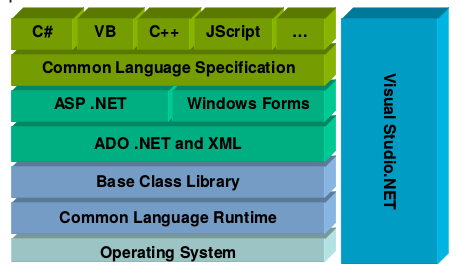
\includegraphics[width=0.5\textwidth]{dot_net}
\end{figure}
\textbf{Common Language Runtime (CLR)} je jádrem (společná báze) pro spouštění kódu všech programovacích jazyků v .NET. CLR nepozná v jakém jazyku byl kód vytvořen. Programy vytvořené pro .NET jsou překládány pro CLR. Výsledkem překladu je tzv. řízený modul (managed module).

\subsubsection*{Řízený modul (managed module)}
Řízený modul je standardní PE (Portable Executable) soubor, potřebující pro běh CLR. Skládá se ze 4 částí:
\begin{itemize}
\item {PE header}: hlavička informující o typu souboru (GUI, CUI, DLL) , času překladu, ...
\item \textit{CLR header}: hlavička interpretovaná CLR a utilitami. Obsahuje
požadovanou verzi CLR, umístění a velikost metadat, zdroje (resources), silná jména (strong names), příznaky, ...
\item \textit{metadata}: tabulky údajů udávající 1) typy a členy definované ve zdrojovém kódu modulu; 2) typy a členy, na něž se zdrojový kód odkazuje (které využívá). Odstraňují potřebu hlavičkových souborů (.h) a knihoven (.lib) pro překlad. Celá informace o typech a členech spolu s kódem v IL je obsažena v modulech. Tuto informaci přímo využívají překladače. Visual Studio .NET je využívá pro IntelliSense (nápovědu během psaní kódu, které členy lze použít a jaké parametry mají dané metody). CLR je využívá pro kontrolu, že kód obsahuje jen „bezpečné“ operace. Jsou užívána pro serializaci dat v paměti, pro přenos na vzdálený počítač a obnovení stavu objektů na vzdáleném počítači. Umožňují garbage collectoru sledovat dobu života (lifetime) objektů. Pro každý objekt může garbage collector určit jeho typ a z metadat zjistí které položky se odkazují na jiné objekty.
\item \textit{Intermediate Language (IL)}: kód generovaný překladačem. Později je tento kód dále CLR překládán do instrukcí procesoru. Je založen na práci se zásobníkem, jeho instrukce vkládají (push) operandy na zásobník a vytahují (pop) výsledky ze zásobníku. Má omezenou množinu instr ukcí a nepracuje přímo s registry procesoru, což zjednodušuje vývoj překladačů. Největším přínosem je robustnost aplikací. Během překladu z IL do instrukcí procesoru CLR provádí tzv. verifikaci. Během ní se zkoumá IL kód, zda vše co provádí je „bezpečné“ (safe).
\end{itemize}

\subsubsection*{Exekuce řízeného IL kódu}
Při zavedení do paměti se pro všechny metody vytvoří náhradní metody (stub). Při prvním zavolání jakékoliv metody skáče náhradní metoda do CLR. CLR načte kód v IL a přeloží metodu do kódu procesoru (native CPU code) pomocí tzv. Just-in-time překladače (JITCompiler). Náhradní metoda je přepsána kódem volajícím přeloženou metodu. Přeložená metoda se zavolá. Při druhém a dalším volání se volá přímo přeložená metoda.

Špatně detekovatelné chyby v programech jsou často spojeny se správou paměti. V jazycích C, C++ často dochází k paměťovým únikům (memory leaks) – paměť se naalokuje, ale neuvolní. Řešení v CLR: Garbage Collector (x cyklické odkazy, časová náročnost). CLR nepracuje přímo s moduly, ale se assembly - logická skupina jednoho nebo několika řízených modulů a zdrojů (resources), nejmenší samostatný kus SW pro instalování, má svou verzi (private/shared assembly).

Typy v CLR (Common Type System - CTS): kód napsaný v jednom jazyku může pomoci nich komunikovat s kódem z jiného jazyka: field, method, property, event. Common Language Specification (CLS): CLR integruje všechny jazyky tak, že objekty vytvořené v jednom z nich mohou být plně využívány v úplně jiném jazyku. CLS definuje minimální množinu rysů, které musí podporovat každý překladač pro CLR.

\subsection{Jazyk C\#: hodnotové a referenční typy; jednoduché typy, implicitní konverze; výrazy a operátory; příkazy; výjimky.}
Datové typy (Types): hodnotové, referenční (odkazové), zabalení a rozbalení

\subsubsection*{Hodnotové typy}
Proměnná hodnotového typu obsahuje hodnotu tohoto typu (např. typ:int, proměnná:v, hodnota:123). Přiřazení vytváří kopii přiřazované hodnoty. Od hodnotových typů nelze dále dědit. Patří mezi ně:
\begin{itemize}
\item struktury (struct): Struktury jsou podobné třídám v tom, že mohou obsahovat datové členy a funkční členy. Na rozdíl od tříd jsou struktury hodnotové typy! Jsou vhodné zejména pro malé objekty, které nevyžadují dědičnost.
\item jednoduché typy: rezervovaná slova (byte, short, int, long, char, float, bool, ...)
\item výčtové typy (enum): deklarují množinu pojmenovaných konstant (pro každý enum je v pozadí nějaký celočíselný typ. Např. enum Color \{Red, Green, Blue\}.
\end{itemize}

\subsubsection*{Referenční typy}
Proměnná referenčního typu obsahuje referenci (odkaz) na instanci typu objekt. Přiřazením do proměnné referenčního typu ukazuje proměnná na stejnou instanci objektu jako přiřazovaná. Referenční typy jsou:
\begin{itemize}
\item třídy (class)
\item rozhraní (interface): Rozhraní definuje „kontrakt“. Třída nebo struktura, implementující interface musí dodržovat tento kontrakt. Interface může dědit z několika bázových interfaců. Interface neimplementuje členy, které definuje. Implementují je třídy nebo struktury, které jsou od daného rozhraní odvozeny.
\item pole (array): Pole jsou datové struktury, k jejichž prvkům se přistupuje pomocí vypočtených indexů. Dimenze pole = počet indexů; jedno a vícedimenzionální pole (dvou, třídimenzionální, ...). Prvkem pole může být libovolný typ, včetně pole.
\item delegáty (delegates): Umožňují implementovat scénáře známé z jazyků C, C++, Pascal, atd. jako ukazatele na funkce. Na rozdíl od C++ (atd.) jsou plně objektově orientovány a zapouzdřují (encapsulates) jak instanci objektu, tak i metodu. Deklarace delegáta definuje třídu odvozenou od System.Delegate a delegáty jsou implicitně sealed. Daná metoda a delegát jsou kompatibilní, mají-li stejný počet parametrů stejných typů ve stejném pořadí a se stejnými
modifikátory parametrů a stejný návratový kód. Delegáty jsou v C\# ekvivalentní podle jména, ne podle struktury deklarace. Dva různé typy delegátů jsou odlišné typy, i když mají shodný seznam parametrů i návratový kód. Seznam volání (invocation list) je posloupnost metod zapouzdřená do instance delegátu.
\end{itemize}

Převod z hodnotového typu na referenční se nazývá zabalení (boxing). Provádí se automaticky, když se hodnotový typ vyskytuje v místě, kde má být object. Opačný převod je rozbalení (unboxing). Je třeba použít explicitní přetypování, typ před zabalením a při rozbalení se musí přesně shodovat! Konverze mezi dvěma typy může být implicitní (long a = b) nebo explicitní (int c = (int) b).

\subsubsection*{Výrazy a operátory}
Výraz je posloupnost operátorů a operandů. Existují 3 druhy operátorů:
\begin{itemize}
\item unární (např. x++)
\item binární (např. x+y)
\item ternární (např. c ? x : y)
\end{itemize}

\subsubsection*{Příkazy}
Patří sem bloky, prázdné příkazy, deklarační příkaz (deklaruje lokální proměnné nebo konstanty), výrazový příkaz (vyhodnocení výrazu), výběrové příkazy (if, switch), iterační příkazy (for, while, do, foreach), skokové příkazy (break, continu, goto, return, throw), příkaz try, příkazy checked a unchecked (určují, jak bude ošetřeno přetečení celočíselných aritmetických operací a konverzí), příkaz lock (realizuje vzájemně výlučný (mutual-exclusive) přístup k danému objektu, vykoná příkaz a přístup uvolní), příkaz using (usnadňuje užívání jmenných prostorů a typů v nich definovaných).

Všechny příkazy kromě příkazů s návěštím a deklaračních příkazů se nazývají vložené (embedded). Vložené příkazy se používají v rámci jiných příkazů.

\subsubsection*{Výjimky}
Výjimky jsou v C\# strukturovaným a typově bezpečným způsobem zpracování systémových i aplikačních chyb. Mohou být vyvolány dvěma způsoby: 1) příkazem throw; 2) Během zpracování příkazů a výrazů jazyka C\#, kdy nějaká operace nemůže být dokončena normálně. Jsou obsluhovány příkazem try.


\subsection{Jazyk C\#: Členy a přístup k nim; jmenné prostory; třídy, metody, vlastnosti, konstruktory, destruktory; struktury; pole; delegáty; atributy.}
\subsubsection*{Členy a přístup k nim}
Jmenné prostory a typy mají členy. Členy dané entity (objektu, jmenného prostoru) jsou dostupné pomocí kvalifikovaného jména: entita.jméno-člena.
\begin{itemize}
\item Jmenný prostor (namespace): členy jsou jmenné prostory a typy deklarované uvnitř něj.
\item Struktura (struct): členy deklarované ve struktuře (např. jednoduché typy) a členy zděděné od třídy object.
\item Vyjmenovaný typ (enum): deklarované konstanty a členy zděděné z třídy System.Enum.
\item Třída (class): deklarované členy v této třídě a členy zděděné od bázové třídy kromě konstruktorů a destruktorů.
\item Rozhraní (interface): deklarované členy v interfacu, členy všech bázových interfaců a členy zděděné od třídy object.
\item Pole (array) : členy zděděné z třídy System.Array
\item Delegát (delegate): členy zděděné z třídy System.Delegate
\end{itemize}
Přístup ke členům je určen v deklaraci pomocí modifikátorů:
\begin{itemize}
\item public: přístup není omezen
\item protected: přístup z typu v němž je deklarace a z odvozených typů
\item internal: přístup omezený na daný program
\item protected internal: přístup omezený na daný program nebo odvozené typy
\item private: přístup omezen na typ, v němž je deklarace uvedena
\end{itemize}

\subsubsection*{Jmenné prostory (Namespaces)}
Kód programů v C\# je organizován do jmenných prostorů (direktiva using). Deklarace jmenného prostoru se může nacházet v nejvyšší úrovni ve zdrojovém souboru (takový jmenný prostor se stává členem globálního jmenného prostoru) nebo se nachází uvnitř (vnitřní jmenný prostor) jiného jmenného prostoru (vnější jmenný prostor). V obou případech musí být jméno jmenného prostoru jedinečné uvnitř jej obsahujícího jmenného prostoru.

\subsubsection*{Třídy (Classes)}
Třída je datová struktura, která může obsahovat: 1) datové členy (konstanty a položky); 2) členské funkce (metody, vlastnosti, události, operátory, konstruktory a destruktory); 3) vnořené typy. Mohou využívat dědičnost (inheritance) - odvozená třída může rozšiřovat a specializovat třídu základní (od sealed nelze odvozovat nové třídy). Modifikátor abstract označuje neúplnou třídu, která je určena pouze jako bázová třída.
\begin{itemize}
\item \textit{Metody}: Člen implementující výpočet nebo akci s danou třídou (objektem). Může mít hodnotové, referenční (odpovídá stejnému místu v paměti jako proměnná, která je argumentem v okamžiku volání) a výstupní parametry. Dále také pole parametrů deklarované modifikátorem params (pole je vždy posledním parametrem). Statické vs. instanční (this) metody. Virtuální metody mohou být nahrazeny odvozenými třídami vs. override metody mění (přebíjí) implementaci existující zděděné virtuální metody. Abstraktní metody zavádí virtuální metodu, ovšem bez implementace - tu musí dodat odvozené třídy. Externí metody (extern) jsou typické implementovány v jiném programovacím jazyku.
\item \textit{Vlastnosti}: Člen umožňující přístup k charakteristikám dané třídy (objektu), např. délka řetězce, velikost fontu, apod.
\item \textit{Konstruktory instancí}: člen implementující akce nezbytné pro inicializaci instance třídy. Nedědí se.
\item \textit{Destruktory}: Člen, implementující akce nezbytné pro zrušení (destrukci) instance dané třídy. Destruktory se nedědí a nelze je volat explicitně. Instance se stává způsobilou pro destrukci, pokud ji nemůže používat žádný kód. Instanci uklízí garbage collector. Nemohou být přetížené (nemají parametry), proto třída může mít nejvýše jeden destruktor.
\item \textit{Atributy}: Deklarace v C\# umožňují používat „značky“ vkládané do zdrojového kódu pro specifikaci „přídavné“ informace. Tuto informaci lze získat při běhu programu pomocí tzv. reflexe. Atributy se vkládají do zdrojového kódu do hranatých závorek [ ].
\item \textit{Indexery}: Člen umožňující, aby byl objekt indexován stejným způsobem jako pole (array).
\end{itemize}

\subsection{Softwarové komponenty: DLL, RPC, COM; interface; OPC.}
\subsubsection*{Dynamicky linkované knihovny (.DLL)}
Moduly obsahující funkce a data. Jsou zaváděny do paměti svými volajícími moduly (.exe nebo .dll) a jsou mapovány do paměti volajícího procesu (programu). Mohou definovat dva druhy funkcí:
\begin{itemize}
\item \textit{exportované funkce} - mohou být volány jinými moduly
\item \textit{interní funkce} - mohou být volány jen uvnitř DLL, kde jsou definovány
\end{itemize}
DLL umožnily rozdělit aplikace do více modulů tak, aby kód mohl být snadněji sdílen a aktualizován. Existují dva způsoby, jak volat funkci z DLL:
\begin{itemize}
\item \textit{Load-time dynamic linking} – modul přímo explicitně volá funkce exportované z DLL. To vyžaduje linkování daného modulu s tzv. import library z DLL, která obsahuje informace o tom, kde leží dané exportované funkce.
\item \textit{Run-time dynamic linking} – modul používá funkci LoadLibrary() nebo LoadLibraryEx() k zavedení DLL knihovny za běhu. Pak volá funkci GetProcAddress() pro získání adres exportovaných funkcí z DLL. Tento způsob nepotřebuje import library.
\end{itemize}

\subsubsection*{Remote Procedure Call (RPC)}
Volání funkcí na vzdáleném počítači v architektuře klient-server. V obvyklých aplikacích architektury klient-server se programátor musí naučit detaily komunikace pro dané sítě včetně způsobu obsluhy chyb, převádět data do různých interních formátů a komunikovat s různými rozhraními.Při použití RPC se nemusí psát žádný kód obsluhující síťovou komunikaci v daném protokolu.

\textbf{Jak RPC funguje?} RPC „se tváří“, jako by klient přímo volal proceduru v programu serveru, ve skutečnosti však volá stejnojmennou proceduru z „Client Stub“:
\begin{itemize}
\item získává parametry z adresového prostoru klienta
\item převádí parametry do standardní reprezentace NDR (network data representation)
\item volá funkce pro RPC z Client Run-Time Library
\end{itemize}
Server pro volání vzdálené procedury dělá:
\begin{itemize}
\item „Server Run-Time Library“ přijme požadavek a zavolá proceduru ze „Server Stub“
\item Tato procedura vyjme parametry z bufferu a převede je z NDR do potřebného tvaru
\item „Server Stub“ zavolá proceduru na serveru
\end{itemize}
Po provedení procedury se výsledná data vrací klientovi obdobným způsobem. RPC je jednou částí DCE (Distributed Computing Environment) - prostředí pro distribuované počítání definované sdružením Open Software Foundation (OSF).

\subsubsection*{Component Object Model (COM)}
\textit{Motivace pro používání komponent}: Monolitické aplikace musely být aktualizovány jako celek, komponentové aplikace mohou se aktualizovat (upgrade) po částech. Komponenta je jakási miniaplikace. Celá aplikace se skládá z pospojovaných komponent („LEGO“). Vylepšování aplikace je často záležitostí nahrazování starých komponent novými.

\textit{Požadavky na komponenty}: dynamické linkování - možnost výměny komponenty za běhu; zapouzdření (encapsulation) - Aby bylo možno nahrazovat komponenty bez nutnosti překladu musí být dodrženo rozhraní (interface) mezi komponentou a jejím klientem (programem, který ji využívá). Jsou dodávány v binární formě a nezveřejňují jazyk, v kterém byly napsány.

\textit{Co je COM?} COM je nástroj, který umožnil „rozbít“ monolitické aplikace na komponenty. COM je specifikace (standard) - říká, jak vytvářet (psát) komponenty, které mohou být dynamicky zaměňovány. COM má své API, tzn COM knihovnu, které poskytuje služby pro práci s komponentami. COM používá DLL, aby komponenty měly schopnost dynamického linkování.

\textit{Historie}: Původní cíl byla podpora koncepce známé jako „Object Linking and Embedding“ (OLE) - např. vložení a editace tabulky Excelu do Wordu.

\textbf{COM Interface (rozhraní}: Interface v COMu je množinou funkcí, které implementuje komponenta a klient je volá. Přesněji, interface je paměťová struktura obsahující pole ukazatelů na funkce. Interface lze reprezentovat obdélníkem s naznačeným vysunutým „jackem“.

\subsubsection*{OLE for Process Control (OPC)}
OPC Foundation - neziskové sdružení, které zavedlo několik standardizovaných protokolů na bázi OLE/COM. Snaha o zlepšení interoperability mezi aplikacemi v oblasti automatizace a řízení, řídicími systémy a kancelářskými aplikacemi v oblasti řízení procesů. Definují standardní objekty, metody a vlastnosti pro servery poskytující informace v reálném čase, např. distribuované řídicí systémy, programovatelné automaty (PLC), inteligentní snímače, apod. Informace se v reálném čase komunikují do zařízení podporujících OLE/COM (servery, aplikace, apod.).

Komunikace prostřednictvím OPC má architekturu Klient-Server. Server poskytuje data, komunikuje s fyzickými zařízeními a klient komunikuje se serverem, který plní jeho požadavky. OPC server poskytuje přístup (čtení, zápis, komunikaci) k množině datových zdrojů (sources). OPC klient se připojuje k OPC serveru a komunikuje s ním prostřednictvím interfaců.

Specifikace OPC obsahují vždy dvě sady interfaců:
\begin{itemize}
\item \textit{Custom interfacy} - základní rozhraní implementovaná OPC servery, poskytují maximální výkon
\item \textit{Automation interfacy} - nepovinná rozhraní, jsou vhodné pro skriptovací jazyky (Visual Basic, Excel, ...)
\end{itemize}
\textit{Kde je OPC vhodné?} OPC je primárně navrženo pro přístup k datům ze síťového serveru. OPC interfacy však mohou být použity na mnoha místech v aplikaci (SCADA). Architektura a návrh OPC dovoluje klientské aplikaci přistupovat k datům z mnoha OPC serverů, mnoha dodavatelů, běžících na různých počítačích v síti prostřednictvím jediného objektu serveru.

\subsection{Operační systémy: procesy a thready, synchronizace, deadlock, inverze priorit; správa paměti; vstupně-výstupní systém, programované vstupy/výstupy, přerušení, DMA, ovladače zařízení; souborové systémy.}

\subsection{Operační systémy reálného času: statické a dynamické plánovací algoritmy.}

\subsection{Struktury vzdálených a virtuálních laboratoří.}

\newpage
\section{Převodníky fyzikálních veličin [PFV]}

\begin{table}[H]
\centering
\begin{tabular}{p{4cm} p{12cm}}
\textit{vyučující:}             & Ing. Libor Jelínek Ph.D. \\
\textit{ročník/semestr studia:} & 4.ročník/LS \\
\textit{datum zkoušky:}         & 16. 6. 2016 \\
\textit{hodnocení:}             & 2 \\
\textit{cíl předmětu (STAG):}   & \\
\multicolumn{2}{p{16cm}}{Cílem předmětu je seznámit studenty se základními principy, vlastnostmi a modely senzorů a akčních členů pro potřeby automatizace, monitorování a diagnostiky.}
\end{tabular}
\end{table}

\subsection{Struktura a parametry senzorů pro automatizaci, statické a dynamické modely a chyby, metody snižování chyb senzorů.}

\subsection{A/D a D/A převodníky, obvody pro úpravu signálů, frekvenční filtry.}

\subsection{Senzory teploty a tepla, obvody pro měření odporu, kapacity, indukčnosti a frekvence.}

\subsection{Senzory polohy a vzdálenosti (odporové, indukční, kapacitní, ultrazvukové, optické).}

\subsection{Senzory síly, hmotnosti, deformace, tlaku, rychlosti, zrychlení a vibrací (tenzometrické, piezoelektrické, kapacitní a elektrodynamické).}

\subsection{Senzory průtoku, množství, hustoty, viskozity, koncentrace a chemického složení.}
\subsubsection*{Senzory průtoku}
Senzory průtoku tekutin (tj. kapalin i plynů) určují množství objemové $ Q_V $ nebo hmotnostní $ Q_m $ tekutiny proteklé zvoleným průřezem za jednotku času.
\begin{itemize}
\item \textit{Plovákové senzory}: Používají plovák pohybující se v kuželovité nádobě jako indikátor rovnováhy sil. Tekutina proudící zespodu nadnáší plovák (drážky na obvodu vyvolávají stabilizační rotaci) a mění se štěrbina mezi nádobkou a plováčkem. Tím klesá tlakový spád na plováčku. K ustálení jeho polohy dojde, když síly působící směrem dolů (gravitační síla zmenšená o vztlak) jsou v rovnováze se sílou působící nahoru (účinek tlakové diference mezi spodní a vrchní plochou plováčku).
\item \textit{Dávkovací senzory}: Využívají přenosu elementárního množství objemu v uzavřených komorách, např. mezi zuby ozubených kol. Jsou to v podstatě varianty rotačních čerpadel. Jako příklad poslouží senzor se dvěma ozubenými oválnými písty, které se otáčejí ve válcových komorách. Je poháněn rozdílem točivých momentů vyvolaných tlaky $ p_1 $ a $ p_2 $ na příslušné průměty činné plochy pístů.
\item \textit{Turbínkové a lopatkové senzory}: Protékající tekutina uvádí do rotačního pohybu soustavu vhodně uspořádaných ploch - pro šroubovicový pohyb optimalizovaných lopatek turbiny nebo plochých lopatek vodního kola. Turbínkové senzory při minimalizaci ztrát třením mají široký rozsah lineární závislosti úhlové rychlosti rotoru $ \omega_r $ na rychlosti proudění $ v $. Úhlová rychlost se snímá počítáním průchodů lopatek pod senzorem polohy. Nejčastěji se užívá senzoru indukčního, v němž změna magnetického toku při otáčení lopatek pod snímací cívkou s permanentním magnetem generuje impulsy napětí.
\item \textit{Vírové senzory}: Vhodně formovaný objekt v cestě proudící tekutiny může vyvolat její oscilační pohyb, jehož parametry jsou úměrné objemovému průtoku. Pro měření průtoku se využívá dvou typů oscilací tekutiny: nucené a přirozené oscilace. Pod nucenými oscilacemi se rozumí generace vírů těsně za žebrovitou překážkou na straně vtoku a jejich spirálový pohyb ve směru proudění. Většina vírových senzorů pracuje však s přirozenými oscilacemi, kdy víry jsou oddělovány za překážkou (střídavě na horní a dolní straně), jelikož proudící tekutina není schopna sledovat tvar překážky (tzv. Kármánovy vírové stezky).
\item \textit{Ultrazvukové senzory}: Jsou založeny na skládání vektoru rychlosti $ v $ tekutiny a ultrazvukové vlny $ c_0 $. Ultrazvuková vlna se od měniče $ (V_2, P_2) $ k měniči $ (V_1, P_1) $ bude šířit rychlostí $ c_0 + v \cdot cos \alpha $ a zmenšenou rychlostí$ c_0 - v \cdot cos \alpha $, když postupuje proti směru $ v $ k měniči $ (V_2, P_2) $
\item \textit{Indukční senzory}: 
\end{itemize}

\subsection{Elektrické akční členy a jejich budiče (stejnosměrné, střídavé, krokové motory, PWM zesilovače, frekvenční měniče).}

\subsection{Hydraulické a pneumatické akční členy (pracovní a řídicí mechanizmy a zdroje tlakového média).}